\documentclass[11pt]{article}
\usepackage[a4paper, margin=1in]{geometry}
\usepackage{graphicx}
\usepackage{amsmath}
\usepackage{booktabs}
\usepackage{hyperref}
\usepackage{caption}
\usepackage{float}
\usepackage{subcaption}

\title{\textbf{Image Classification on CIFAR-100}}
\author{}
\date{}

\begin{document}

\maketitle

\section{Introduction}

Image classification is a fundamental task in computer vision where the goal is to assign labels to images based on their visual content. The CIFAR-100 dataset provides a challenging benchmark for evaluating classification algorithms, consisting of 60,000 images across 100 classes, with high intra-class variability.

In this project, we explore and evaluate the performance of various machine learning and deep learning models for image classification on the CIFAR-100 dataset. These models include conventional CNNs, residual and densely connected networks, and transformer-based architectures. We also investigate the impact of pre-training, consistent input preprocessing, and model-specific hyperparameter configurations on classification performance.

\section{Results}

Table \ref{tab:results} summarizes the classification performance of the models using standard evaluation metrics.

\begin{table}[H]
\centering
\caption{Performance comparison of models on CIFAR-100}
\label{tab:results}
\begin{tabular}{lcccc}
\toprule
\textbf{Model} & \textbf{Top-1 Accuracy} & \textbf{Precision} & \textbf{Recall} & \textbf{F1-Score} \\
\midrule
ConvNeXt            & 88.32\% & 88.93\% & 88.32\% & 88.35\% \\
Vision Transformer  & 89.86\% & 90.43\% & 89.86\% & 89.87\% \\
Swin Transformer    & 89.08\% & 89.56\% & 89.08\% & 89.08\% \\
EfficientNetB0      & 84.74\% & 85.16\% & 84.74\% & 84.77\% \\
DenseNet121         & 81.47\% & 82.27\% & 81.47\% & 81.58\% \\
Custom CNN          & 47.27\% & 49.24\% & 47.27\% & 46.06\% \\
ResNet18            & 80.05\% & 80.31\% & 80.05\% & 80.09\% \\
VGG16               & 72.09\% & 73.92\% & 72.09\% & 72.03\% \\
\bottomrule
\end{tabular}
\end{table}

% ====================== Full Confusion Matrices (Part 1) ======================
\begin{figure}[htbp]
\centering
\captionsetup[subfigure]{labelformat=empty}

% First row
\begin{subfigure}[b]{0.48\textwidth}
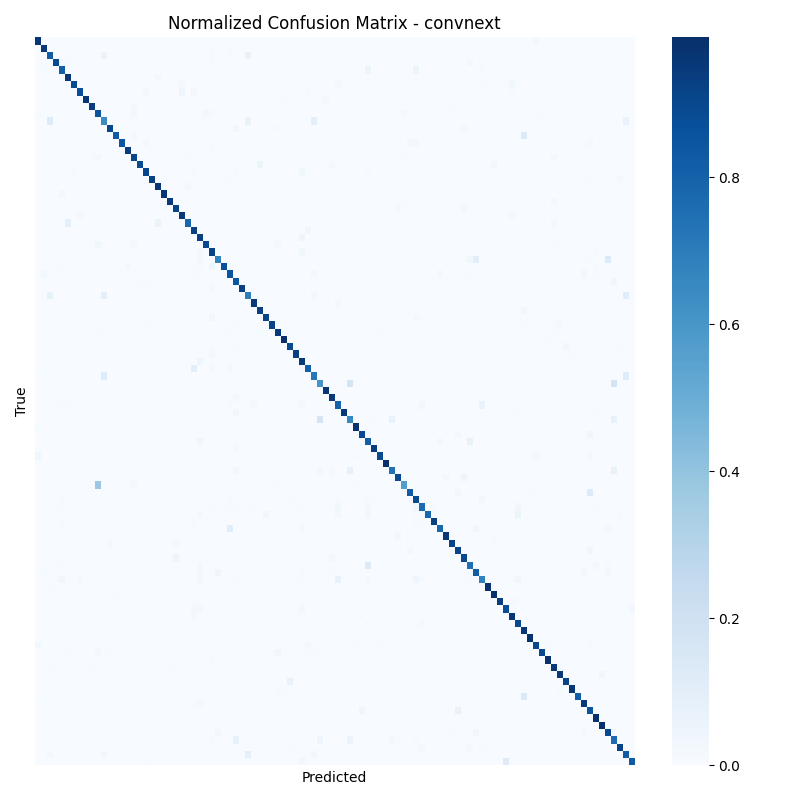
\includegraphics[width=\textwidth]{confusion_matrix_convnext_full.png}
\caption{ConvNeXt}
\end{subfigure}
\hfill
\begin{subfigure}[b]{0.48\textwidth}
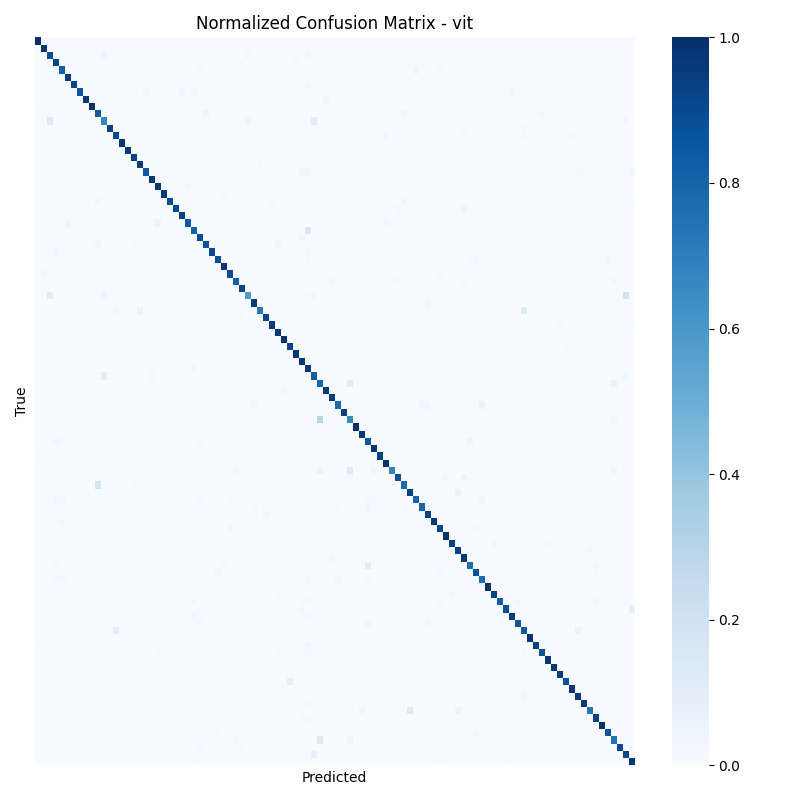
\includegraphics[width=\textwidth]{confusion_matrix_vit_full.png}
\caption{Vision Transformer}
\end{subfigure}

\vspace{0.2cm} % Minimal spacing

% Second row
\begin{subfigure}[b]{0.48\textwidth}
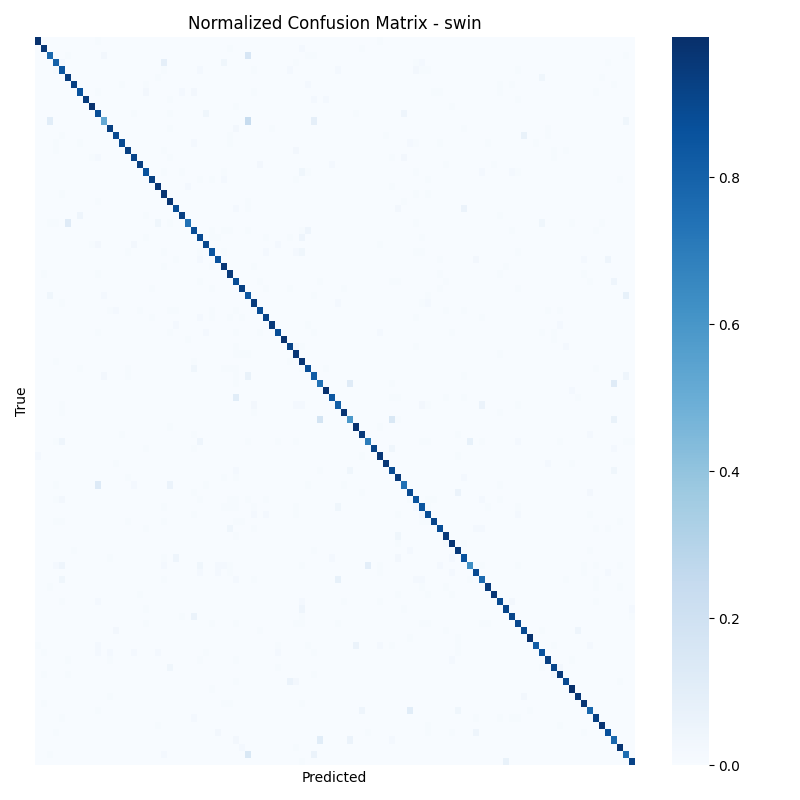
\includegraphics[width=\textwidth]{confusion_matrix_swin_full.png}
\caption{Swin Transformer}
\end{subfigure}
\hfill
\begin{subfigure}[b]{0.48\textwidth}
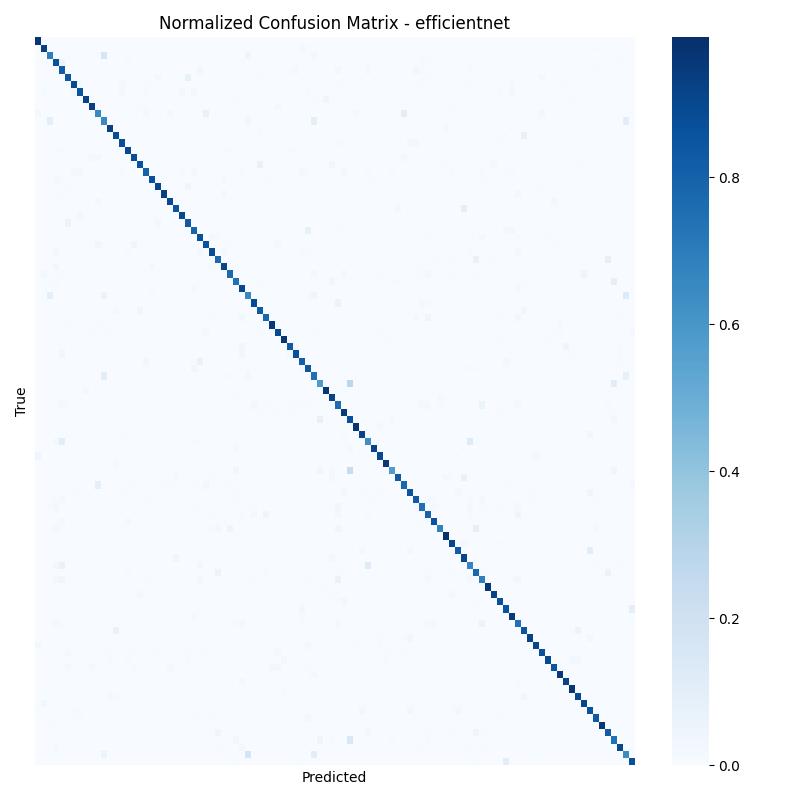
\includegraphics[width=\textwidth]{confusion_matrix_efficientnetb0_full.png}
\caption{EfficientNetB0}
\end{subfigure}

\caption{Confusion matrices (Part 1): High-performance models.}
\label{fig:confusion_part1}
\end{figure}

% ====================== Full Confusion Matrices (Part 2) ======================
\begin{figure}[htbp]
\centering
\captionsetup[subfigure]{labelformat=empty}

% Third row
\begin{subfigure}[b]{0.48\textwidth}
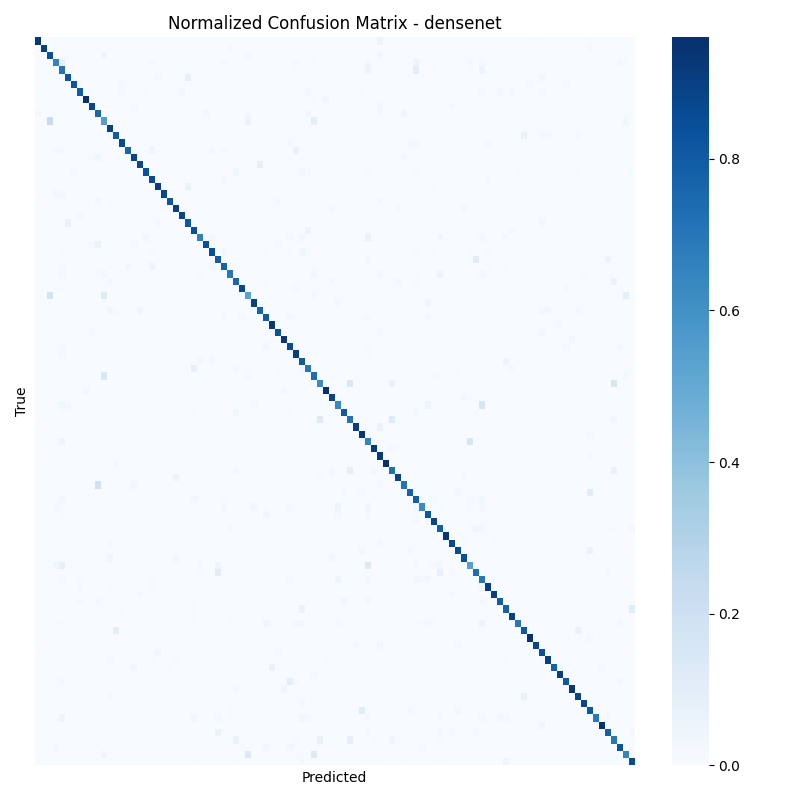
\includegraphics[width=\textwidth]{confusion_matrix_densenet121_full.png}
\caption{DenseNet121}
\end{subfigure}
\hfill
\begin{subfigure}[b]{0.48\textwidth}
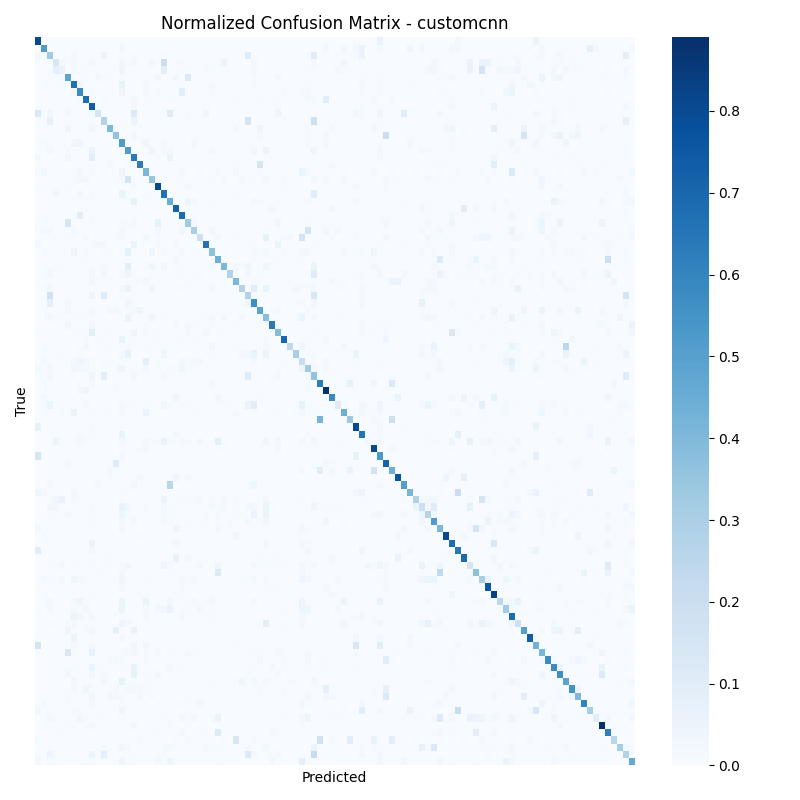
\includegraphics[width=\textwidth]{confusion_matrix_customcnn_full.png}
\caption{Custom CNN}
\end{subfigure}

\vspace{0.2cm}

% Fourth row
\begin{subfigure}[b]{0.48\textwidth}
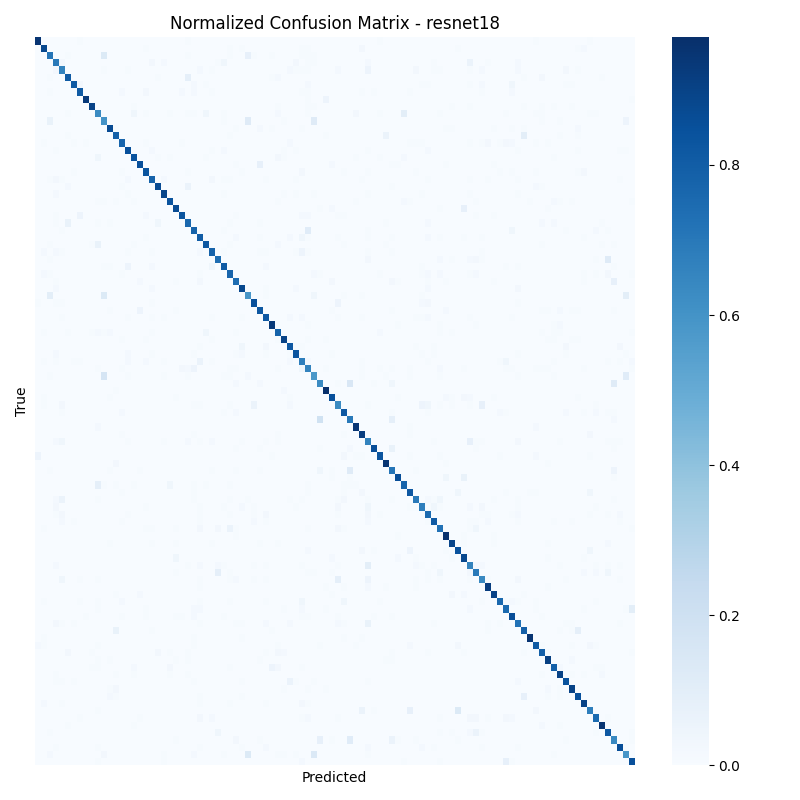
\includegraphics[width=\textwidth]{confusion_matrix_resnet18_full.png}
\caption{ResNet18}
\end{subfigure}
\hfill
\begin{subfigure}[b]{0.48\textwidth}
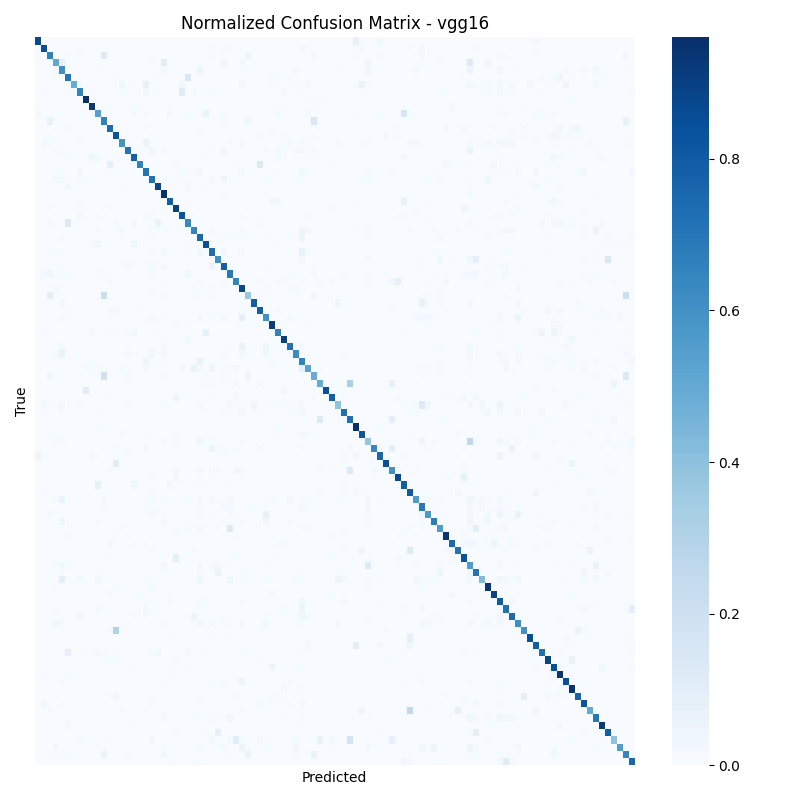
\includegraphics[width=\textwidth]{confusion_matrix_vgg16_full.png}
\caption{VGG16}
\end{subfigure}

\caption{Confusion matrices (Part 2): Moderate and lower-performance models.}
\label{fig:confusion_part2}
\end{figure}

% ====================== Top Confused Classes (Part 1) ======================
\begin{figure}[htbp]
\centering
\captionsetup[subfigure]{labelformat=empty}

\begin{subfigure}[b]{0.48\textwidth}
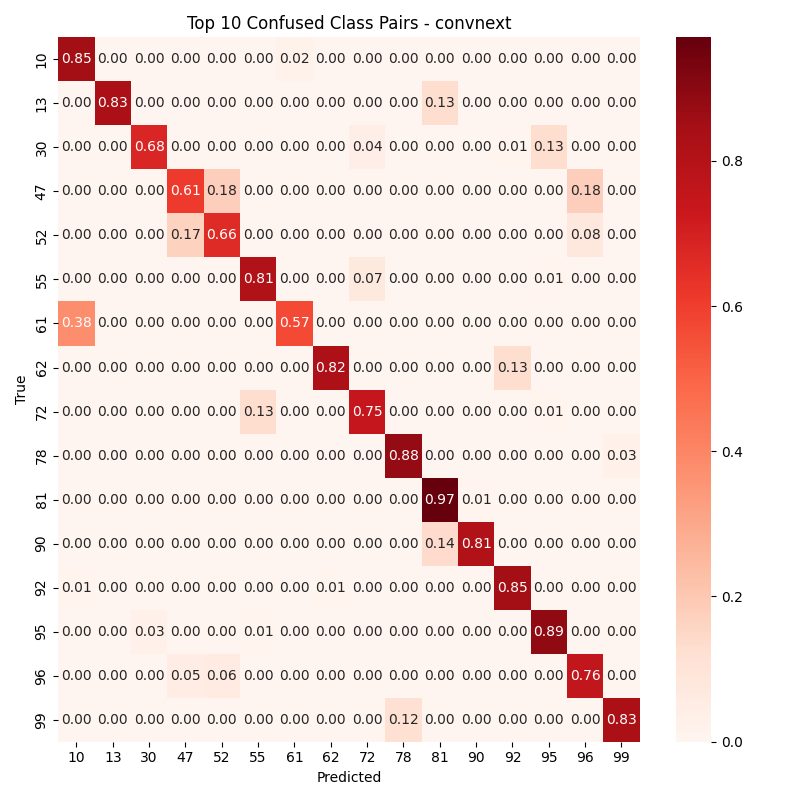
\includegraphics[width=\textwidth]{confusion_matrix_convnext_top_confused.png}
\caption{ConvNeXt}
\end{subfigure}
\hfill
\begin{subfigure}[b]{0.48\textwidth}
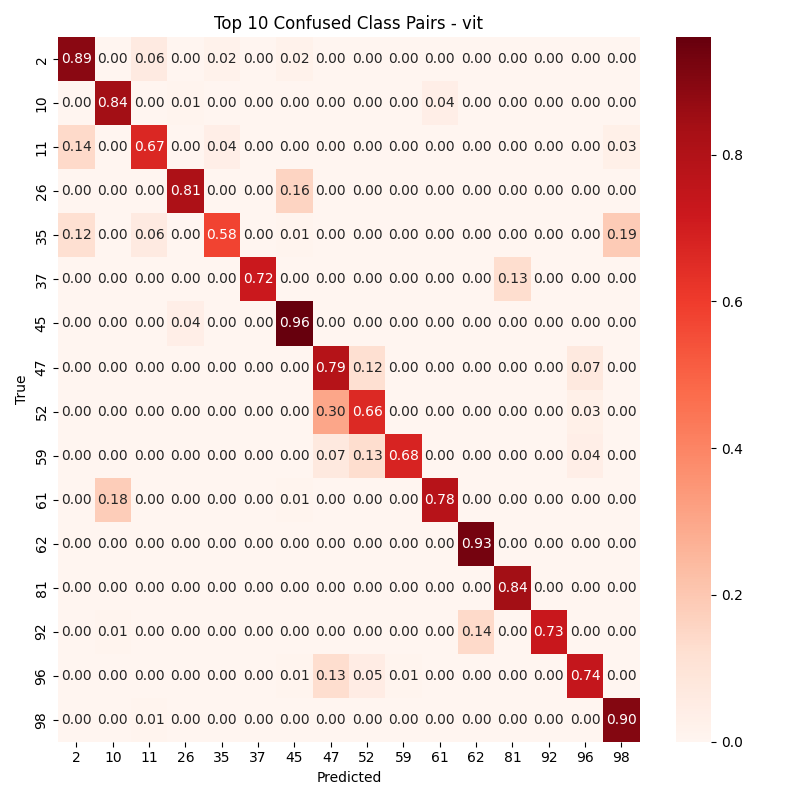
\includegraphics[width=\textwidth]{confusion_matrix_vit_top_confused.png}
\caption{Vision Transformer}
\end{subfigure}

\vspace{0.2cm}

\begin{subfigure}[b]{0.48\textwidth}
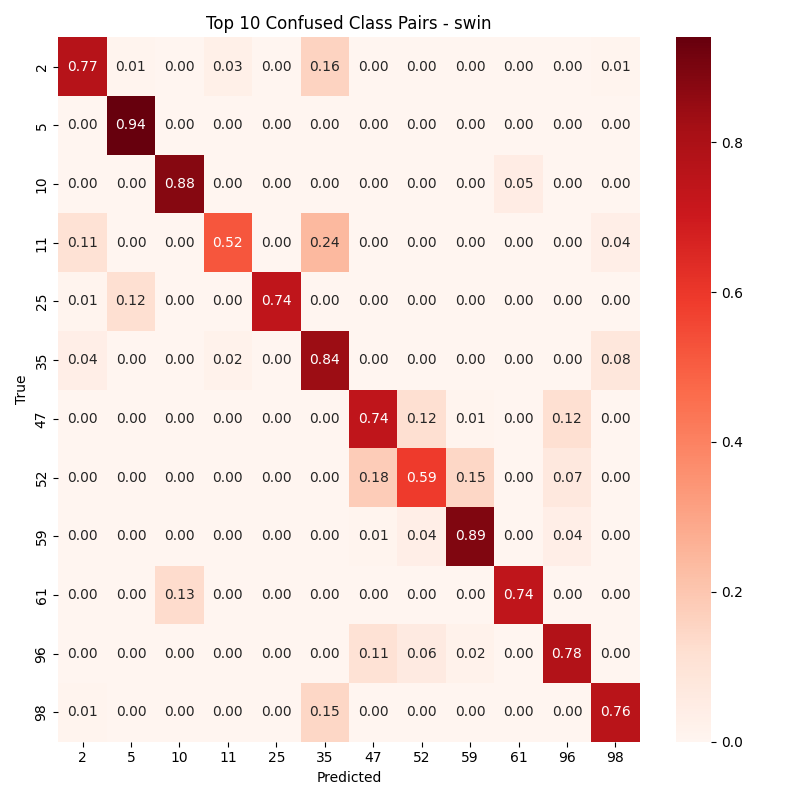
\includegraphics[width=\textwidth]{confusion_matrix_swin_top_confused.png}
\caption{Swin Transformer}
\end{subfigure}
\hfill
\begin{subfigure}[b]{0.48\textwidth}
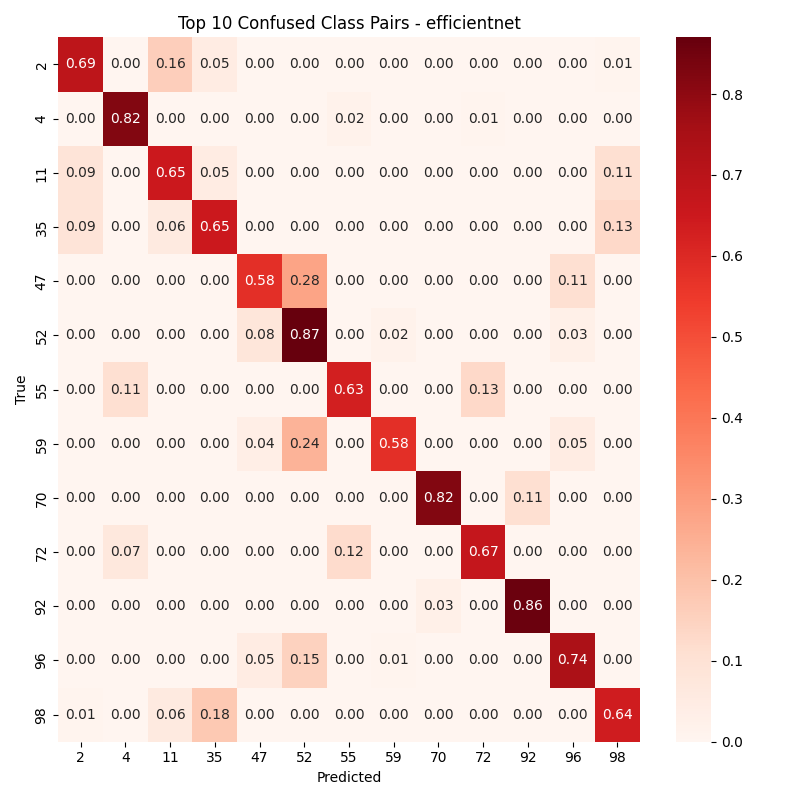
\includegraphics[width=\textwidth]{confusion_matrix_efficientnetb0_top_confused.png}
\caption{EfficientNetB0}
\end{subfigure}

\caption{Top confused classes (Part 1).}
\label{fig:top_confused_part1}
\end{figure}

% ====================== Top Confused Classes (Part 2) ======================
\begin{figure}[htbp]
\centering
\captionsetup[subfigure]{labelformat=empty}

\begin{subfigure}[b]{0.48\textwidth}
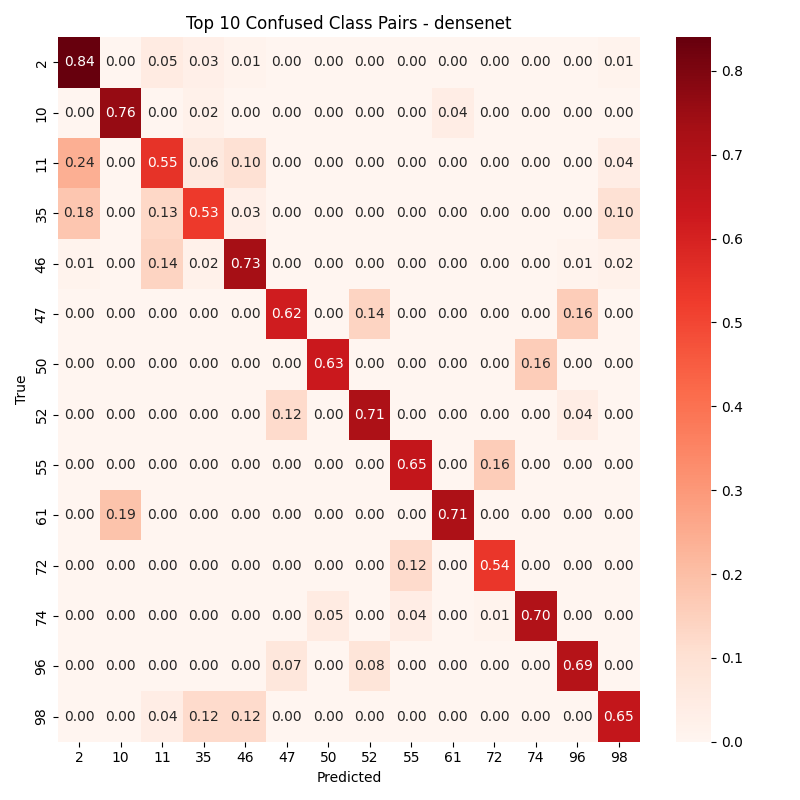
\includegraphics[width=\textwidth]{confusion_matrix_densenet121_top_confused.png}
\caption{DenseNet121}
\end{subfigure}
\hfill
\begin{subfigure}[b]{0.48\textwidth}
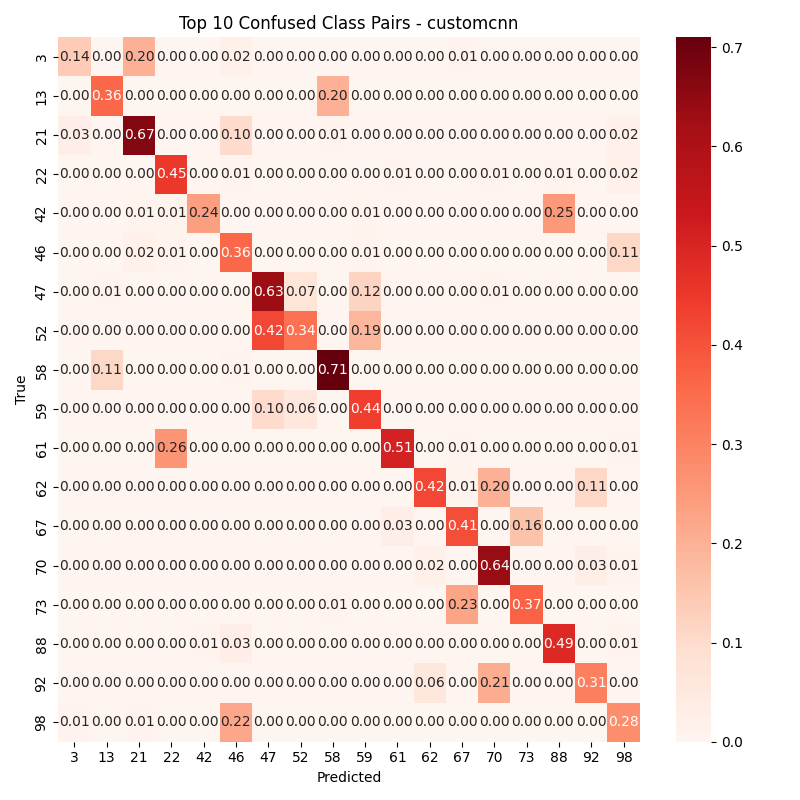
\includegraphics[width=\textwidth]{confusion_matrix_customcnn_top_confused.png}
\caption{Custom CNN}
\end{subfigure}

\vspace{0.2cm}

\begin{subfigure}[b]{0.48\textwidth}
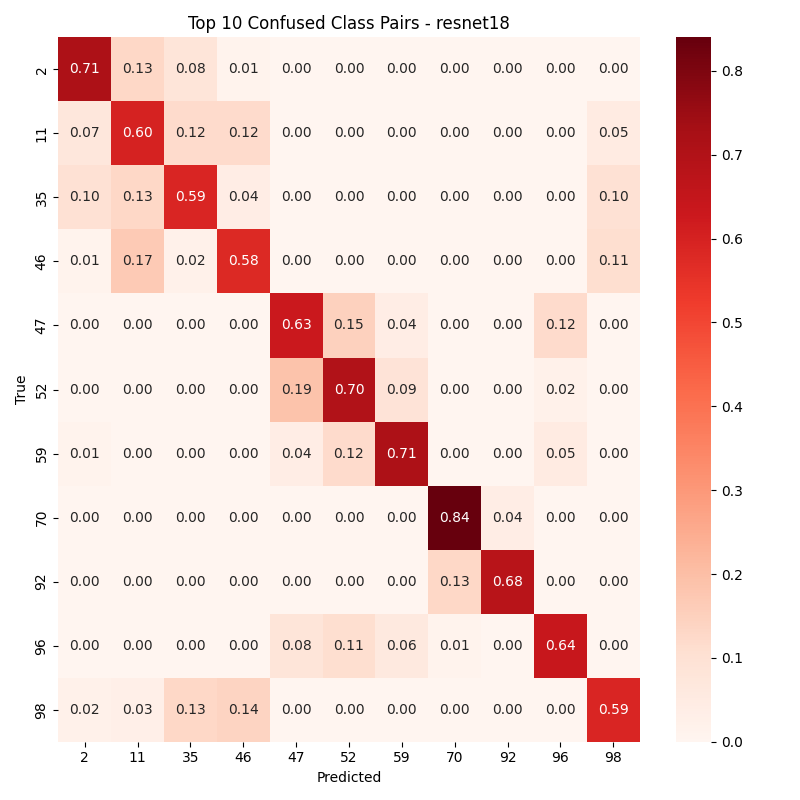
\includegraphics[width=\textwidth]{confusion_matrix_resnet18_top_confused.png}
\caption{ResNet18}
\end{subfigure}
\hfill
\begin{subfigure}[b]{0.48\textwidth}
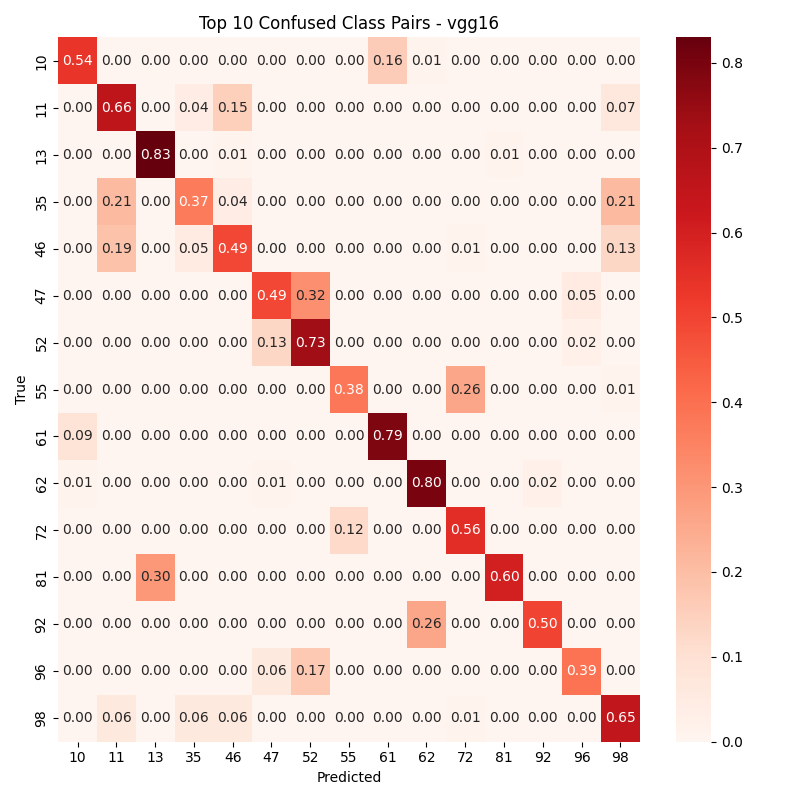
\includegraphics[width=\textwidth]{confusion_matrix_vgg16_top_confused.png}
\caption{VGG16}
\end{subfigure}

\caption{Top confused classes (Part 2).}
\label{fig:top_confused_part2}
\end{figure}

\section{Discussion}

\subsection*{Model Comparison}
Among the evaluated models, the Vision Transformer (ViT) achieved the highest classification accuracy of 89.86\%, closely followed by the Swin Transformer and ConvNeXt. All these high-performing models were pretrained on large datasets (ImageNet-21K and ImageNet-22K). EfficientNetB0 and DenseNet121 showed competitive results with good generalization capabilities, leveraging pretrained weights from ImageNet-1K. ResNet18 and VGG16 performed reasonably well, while the Custom CNN lagged significantly behind due to its simpler architecture and lack of pretraining, despite having a deeper structure with six convolutional blocks.

\subsection*{Hyperparameter Tuning}
Our hyperparameter configurations across different models revealed:
\begin{itemize}
    \item Learning rates: Most models were fine-tuned with a learning rate of $10^{-4}$, while the Custom CNN used a higher learning rate of $10^{-3}$.
    \item Batch sizes: Varied based on model size and memory requirements - from 56 for larger models like ConvNeXt and Swin, 96 for ViT and DenseNet, 128 for ResNet18 and Custom CNN, 164 for EfficientNet, and 64 for VGG16.
    \item Optimizer: Adam optimizer with $\epsilon=10^{-9}$ was used consistently across all models.
    \item Training duration: Ranged from 6 epochs for transformer-based models (ViT, Swin, ConvNeXt) to 16-31 epochs for CNN-based models, allowing adequate convergence for each architecture.
\end{itemize}

\subsection*{Data Augmentation}
Data preprocessing was implemented through a custom dataset class that applied consistent transformations across all models, including:
\begin{itemize}
    \item Image resizing to model-specific input dimensions (224×224 pixels for all models).
    \item Normalization using ImageNet mean (0.485, 0.456, 0.406) and standard deviation (0.229, 0.224, 0.225) values.
\end{itemize}
This standardized approach allowed for fair comparison across all model architectures while ensuring optimal input for pretrained networks.

\subsection*{Visualization and Interpretability}
\begin{itemize}
    \item Misclassified images often belonged to visually similar classes.
    \item CNNs showed meaningful filter activations, highlighting the learned feature hierarchies.
\end{itemize}

\section{Conclusion}

This project evaluated various deep learning architectures on the CIFAR-100 dataset. Key findings include:
\begin{itemize}
    \item Pretrained transformer models (ViT from Google and Swin from Microsoft) achieved the best performance, with ViT leading slightly.
    \item ConvNeXt also provided strong performance with fewer parameters than ViT.
    \item Consistent input preprocessing and model-specific hyperparameter configurations are crucial for maximizing performance.
    \item Fine-tuning pretrained models is more efficient than training from scratch, as evidenced by the Custom CNN's significantly lower performance.
\end{itemize}

Future work may explore ensemble methods, semi-supervised learning, or contrastive pretraining strategies to further improve performance.

\section*{References}

\begin{itemize}
    \item CIFAR-100 Dataset: \url{https://www.cs.toronto.edu/~kriz/cifar.html}
    \item ResNet: He et al., 2015. Deep Residual Learning for Image Recognition.
    \item Vision Transformer: Dosovitskiy et al., 2020.
    \item PyTorch Documentation: \url{https://pytorch.org}
    \item TensorFlow Documentation: \url{https://www.tensorflow.org}
\end{itemize}

\end{document}
